\begin{figure}
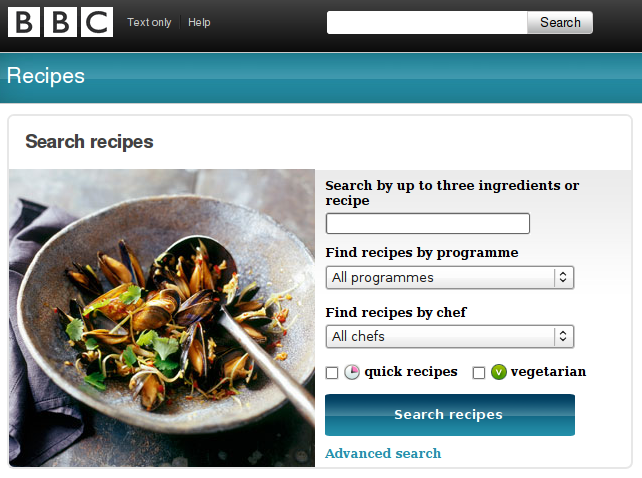
\includegraphics[width=0.9\textwidth]{screenshot_bbc_recipes}
\caption{The BBC Food Recipe Search Page}
\label{fig:bbc_food}
\end{figure}

"You arrive home after a long day at work, open the fridge to find ... a single egg, one lonely onion and some almost mouldy cheese ..." The aim of this project is to develop a software kitchen assistant tool. This tool must be able to provide recipes which match a supplied list of available ingredients. This is similar to the BBC's recipe search\footnote{\url{http://www.bbc.co.uk/food/recipes/}} (Fig~\ref{fig:bbc_food}), but is not constrained to just three search items. The software should provide a number of matching recipes and rank the suggestions according to how well they match. The recipe database can be online and community maintained and take into account the user's own food preferences. To achieve this, collaborative filtering technology can be used to provide and manage the recommendations. Possibly, the lists of required ingredients for a recipe can be exported to a mobile phone as a shopping list. In addition, there is the potential to link the software to an online supermarket such as tesco.com to calculate the current cost of each created meal.
